\documentclass[a4paper, oneside, final]{scrartcl}

\usepackage{scrlayer-scrpage}
\usepackage{titlesec}
\usepackage{marvosym}
\usepackage{tabularx,colortbl}
\usepackage{ebgaramond}
\usepackage{microtype}
\usepackage{hyperref}
\usepackage{graphicx}

\titleformat{\section}{\large\scshape\raggedright}{}{0em}{}[\titlerule]

\pagestyle{scrheadings}

\addtolength{\voffset}{-0.5in}
\addtolength{\textheight}{3cm}

\newcommand{\gray}{\rowcolor[gray]{.90}}

\renewcommand{\headfont}{\normalfont\rmfamily}

\begin{document}

\begin{center}
  {\fontsize{10}{10}\selectfont\scshape\textls[50]{Especificaciones Técnicas}}\\
  {\fontsize{10}{10}\selectfont\scshape\textls[50]{Pizarra Colaborativa para
      Computólogos}}\\
  \vspace{1cm}
  {\fontsize{9}{9}\selectfont\scshape\textls[50]{Equipo 1}}\\
  \vspace{0.2cm}
  {\fontsize{7}{7}\selectfont\scshape\textls[50]{Diego Sebastián Sánchez Correa}}\\
  {\fontsize{7}{7}\selectfont\scshape\textls[50]{Mauro Emiliano Chávez Zamora}}\\
  {\fontsize{7}{7}\selectfont\scshape\textls[50]{Ulises Josué Anaya Pérez}}\\
  {\fontsize{7}{7}\selectfont\scshape\textls[50]{Daniel Linares Gil}}\\
  {\fontsize{7}{7}\selectfont\scshape\textls[50]{Karyme Ivette Azpeitia García}}\\
\end{center}
\vspace{2cm}

\begin{flushright}
  \footnotesize{Creado: 15/02/2024}\\
  \footnotesize{Última vez actualizado: 18/02/2024}\\
\end{flushright}

\section{Resumen}

Se pretende proporcionar una herramienta básica que busca satisfacer las
necesidades esenciales para el desarrollo de proyectos relacionados con las
ciencias de la computación.\\

La idea de un editor de texto con \textit{syntax highlighting} es común dentro
del ámbito de desarrollo de software, sin embargo, se carece de herramientas de
planeación colaborativa donde las ideas se puedan aterrizar de manera general o
con detalles tan específicos como los usuarios lo deseen.\\

Esta aplicación tiene como fin la creación de un ambiente colaborativo y cuya
esencia funja como punto de partida para la elaboración de decisiones de diseño
a partir de diagramas, control de versiones, edición con dibujo vectorizado y
soporte para \LaTeX.

\section{Glosario}

\section{Contexto}

\textbf{Ejemplos de herramientas de pizarra colaborativa}

\begin{itemize}
\item \href{https://miro.com/}{Miro}
\item \href{https://www.mural.co/}{Mural}
\item \href{ https://www.microsoft.com/en-us/microsoft-365/microsoft-whiteboard/digital-whiteboard-app}{Microsoft Whiteboard}
\item \href{https://www.figma.com/figjam/}{Figjam}
\item \href{https://jamboard.google.com}{Jamboard}

\end{itemize}

\textbf{Ejemplos de uso:}

\begin{itemize}
\item \textbf{Entrevista de programación:} Alice se encuentra entrevistando candidatos para unirse a su equipo como
  desarrolladores de software. Alice decide utilizar nuestra pizarra colaborativa porque permite bloques de código,
  dibujar de manera libre y escribir diagramas para explicar la solución. Durante la entrevista, el candidato escribe
  su solución en el bloque de código y además puede utilizar las funcionalidades de diagramado y dibujo libre para explicar su solución a Alice.

\item \textbf{Reunión de retrospectiva:} Alice se prepara para la reunión de retrospectiva de su equipo de desarrollo luego de un sprint. Alice crea una nueva pizarra, y la divide en tres columnas:

  \begin{itemize}
  \item ¿Qué fue bien?
  \item ¿Qué no fue bien?
  \item ¿Qué se puede mejorar?
  \end{itemize}

  Una vez termina de preparar la pizarra, crea un enlace para compartir la pizarra y lo comparte con los miembros de su equipo. Durante la reunión, los miembros del equipos colaboran añadiendo notas en cada columna. Los miembros del equipo
  pueden incluir enlaces a los tickets de Jira correspondientes en las notas. Una vez terminan de añadir notas, los miembros del equipo discuten sobre estas.
\end{itemize}

\clearpage
\section{Requerimientos Técnicos}

\begin{enumerate}
\item \textbf{Integración de Diagramas y Codificación}\\ %diego
  Provee un ambiente donde los desarrolladores pueden crear diagramas y escribir
  código en el mismo lugar, facilitando con ello la visualización y la
  implementación simultánea de ideas.

  Desde conceptos matemáticos simples como la incorporación de autómatas, hasta
  la integración de diagramas de flujo permitirán que los usuarios puedan ser
  capaces de definir las bases, algoritmos y diseño de un proyecto cuya esencia
  tenga una naturaleza colaborativa.

  \begin{figure}[h!]
    \centering
    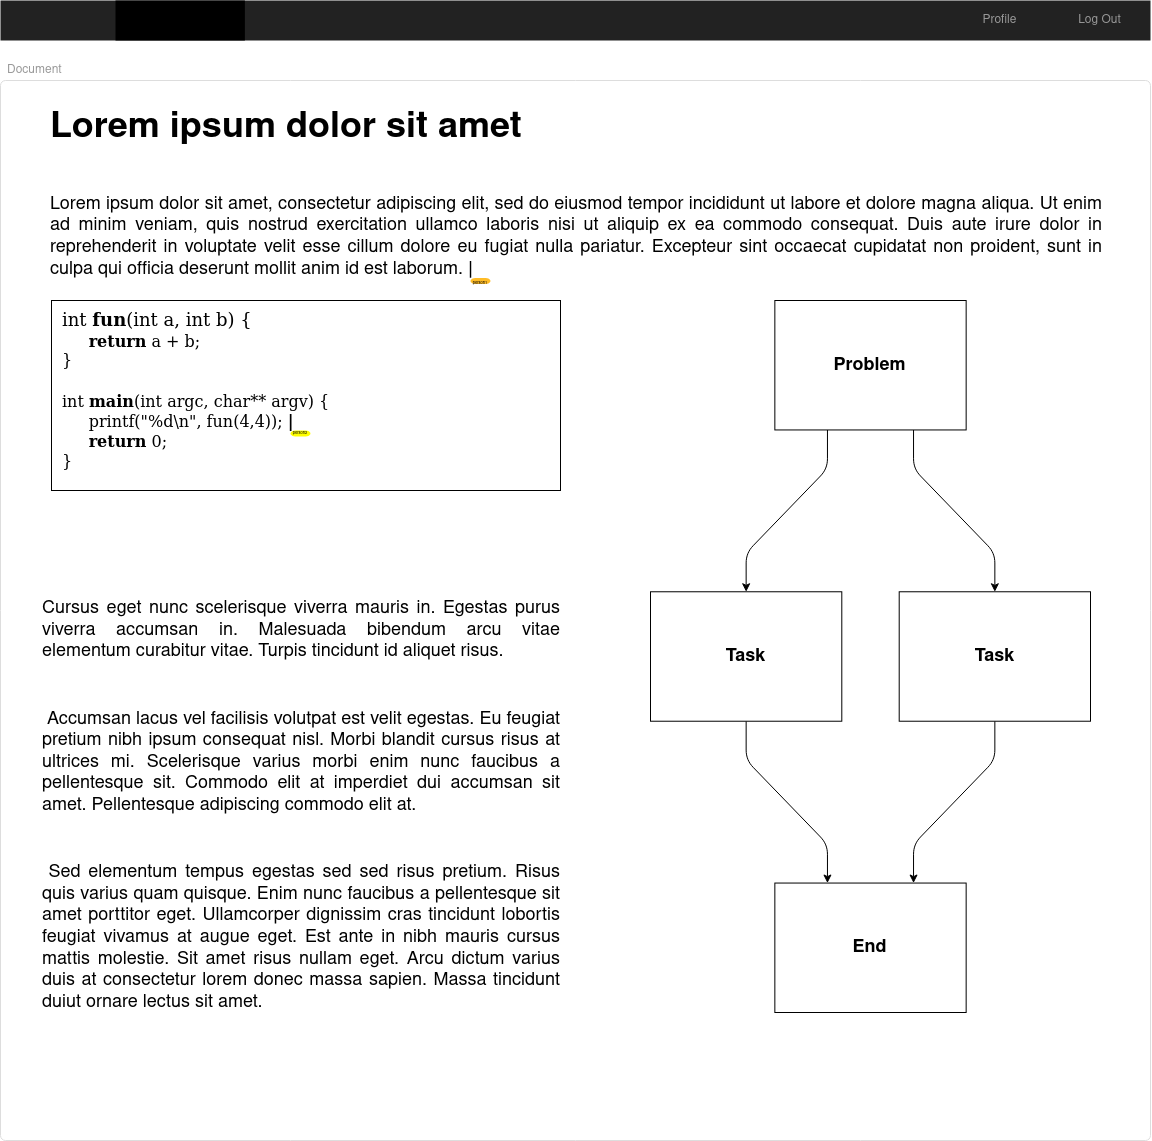
\includegraphics[width=0.88\textwidth]{Interface01.png}
  \end{figure}

  \begin{itemize}
  \item \textbf{Planeación de proyectos de software}: al adjuntar código que esté
    relacionado con diagramas de flujo que representen el problema a resolver y las
    tareas (o proposiciones) asociadas para su compleción, o que denoten cómo estará
    organizado las funciones del programa (incluyendo con ello descripciones
    breves).
  \item \textbf{Editor de notas}: La organización en diagramas ayuda a que funja como una
    aplicación para tomar notas cómoda y fácil de usar. Además, la incorporación de
    formatos para código, hace de esta una herramienta esencial para estudiantes
    de carreras que estén relacionadas con el desarrollo de software.
  \item \textbf{Depuración de código colaborativo}: La visualización colaborativa en
    diagramas del código escrito trae consigo una depuración rápida y básica para
    código no compilado que pretende plantear una idea inicial para dar solución
    a un problema.
  \end{itemize}

  \clearpage
\item \textbf{Colaboración Concurrente}\\ %daniel
  \textbf{Motivación:} El objetivo de la pizarra es fomentar la colaboración y el intercambio de ideas entre usuarios, para lo
  cual es fundamental que la pizarra permita la colaboración en tiempo real entre los usuarios.

  \textbf{Objetivo:} Permitir que múltiples usuarios trabajen de manera simultanea en la pizarra.
  \begin{itemize}
  \item \textbf{Compartir con enlace:} El usuario debe poder generar un enlace único para compartir la pizarra con otros usuarios.

    Solo los usuarios autenticados deben poder acceder a los enlaces. Si un usuario que no se encuentra autenticado o no posee una cuenta intenta acceder a un enlace, será dirigido al flujo de autenticación/registro y luego a la pizarra.

    El usuario debe poder elegir el nivel de acceso que se concede a los usuarios con el enlace:
    \begin{itemize}
    \item \textbf{Solo lectura:} Permite a los usuarios con el enlace ver la pizarra, pero no realizar cambios.
    \item \textbf{Edición:} Permite a los usuarios con el enlace ver y editar la pizarra.
    \end{itemize}

    El usuario debe poder revocar el acceso a la pizarra en cualquier momento.

  \item \textbf{Visualización de la colaboración:} Los usuarios que se encuentren trabajando en una pizarra deben poder visualizar en tiempo real las modificaciones realizadas a la pizarra por otros usuarios.

    \begin{itemize}
    \item \textbf{Indicador de presencia:} Los usuarios deben poder ver en la barra superior los avatares de los usuarios que están conectados a la pizarra.
    \item \textbf{Cursor en tiempo real:} Los usuarios deben poder ver los cursores de los demás usuarios en la pizarra para indicar dónde están trabajando.
    \end{itemize}
  \end{itemize}


\item \textbf{Guardado Automático y Control de Versiones}\\ %kary
  % Garantiza la seguridad de los datos mediante el guardado automático del
  % trabajo hecho en la pizarra; además, ofrece funcionalidades de control de
  % versiones para rastrear y administrar cambios.
  Estas funcionalidades son esenciales para garantizar la seguridad de los datos, facilitar la colaboración y mejorar la productividad de los usuarios. A continuación se describen las especificaciones funcionales.
  \begin{itemize}
  \item  \textbf{Guardado Automático}\\
    El guardado automático protegecontra la pérdida de datos en caso de fallos del sistema, errores del usuario o eventos inesperados.
    \begin{itemize}
    \item \textbf{Frecuencia:} El trabajo del usuario en la pizarra se debe guardar automáticamente con una frecuencia configurable.\\
      \textbf{Opciones de frecuencia recomendadas:}
      \begin{itemize}
      \item Cada 5 minutos
      \item Cada 10 minutos
      \item Cada 15 minutos
      \item Personalizado
      \end{itemize}
    \item \textbf{Ubicación del archivo:} Los archivos guardados automáticamente se deben almacenar en un servidor seguro y accesible para el usuario.
      \begin{itemize}
      \item Opciones de ubicación recomendadas:
        \begin{itemize}
        \item Nube privada(por ejemplo, Google Drive, Dropbox)
        \item Servidor local
        \item Almacenamienro propio de la aplicación
        \end{itemize}
      \end{itemize}
    \item\textbf{Notificaciones:}El usuario debe recibir una notificación cada vez que se guarde automáticamente su trabajo.
      \begin{itemize}
      \item La notificación indicará: Fecha y hora del guardado, asi como ubicación del archivo guardado.
      \end{itemize}
    \end{itemize}
  \item \textbf{Control de Versiones}\\
    El control de versiones permite a los usuarios trabajar juntos en la misma pizarra virtual de forma eficiente. Permite rastrear los cambios, deshacer errores y restaurar versiones anteriores.
    \begin{itemize}
    \item \textbf{Historial de versiones:}El usuario debe poder acceder al historial de versiones y ver las diferencias entre cada versión.
      \begin{itemize}
      \item Opciones para acceder al historial de versiones:
        \begin{itemize}
        \item Lista de versiones con fecha y hora
        \item Miniaturas visuales de cada versión
        \item Deslizador para comparar dos versiones
        \end{itemize}
      \end{itemize}
    \item \textbf{Restauración de versiones:} El usuario debe poder restaurar una versión anterior de la pizarra en cualquier momento.
      \begin{itemize}
      \item Opciones para restaurar una versión:
        \begin{itemize}
        \item Seleccionar una versión de la lista de versiones
        \item Usar un atajo de teclado
        \item Botón de "Restaurar" en la barra de herramientas
        \end{itemize}
      \end{itemize}
    \item \textbf{Revertir cambios:} El usuario debe poder deshacer los últimos cambios realizados en la pizarra.
      \begin{itemize}
      \item Opciones para deshacer cambios:
        \begin{itemize}
        \item Botón de "Deshacer" en la barra de herramientas
        \item Atajo de teclado
        \end{itemize}
      \end{itemize}
    \end{itemize}
  \end{itemize}

\item \textbf{Pizarra Infinita}\\ %mauro
  \textbf{Motivación:} Al momento de trabajar en múltiples pizarras puede ser sencillo que se pierda información relevante durante los cambios de pizarra, si bien lo ideal sería que los temas pudieran agruparse en una pizarra en específico cada uno, hay temas que requerirán más espacio debio a los múltiples elementos que pueden componer una tarea/tema con muchos componentes o pasos.

  \textbf{Objetivo:} Que nuestra aplicación pueda simular una pizarra que nunca se termina conforme las personas van aumentando los elementos que componen su proyecto (notas, inserciones de Latex, etc.) Si bien el generar una pizarra infinita es imposible de manera práctica, deseamos que el espacio brindado sea al menos lo suficientemente grande para que la persona usuaria tenga la sensación de que no estará limitada por las herramientas.

  \begin{itemize}
  \item \textbf{Opciones para implementarla:}

    \begin{itemize}
    \item Que la aplicación tenga un umbral donde detecte qué tanto algunos elementos se han alejado del centro inicial de la pantalla para irle ofrecienco espacio al usuario conforme incorpora más elementos.

    \item Que el usuario pueda solicitar espacio a demanda conforme elige qué sitios del proyecto conviene ampliar en una determinada dirección, de manera que las personas pueda elegir qué tanto van a requerir de la aplicación.

    \item Una combinación de ambas, donde sólo se amplie aquellos lugares de la pizarra donde se estén agregando elementos que se acerquen al límite establecido hasta el momento.
    \end{itemize}
  \end{itemize}

  Como características adicionales, podemos lanzar un aviso cuando una pizarra esté siendo demasiado grande de manera que se sugiera al usuario segmentar el tema para llevar un mejor control del mismo.

\item \textbf{Registro de Usuarios} %ulises
  \begin{itemize}
  \item \textbf{Objetivo:} Permite que los desarrolladores puedan crear su cuenta con un correo electronico y contrasena, de esta manera podran acceder a su pizarra y a sus datos guardados.
  \item \textbf{Funcion:} Los usuarios deben ser capaces de poder registrarse en la apliacion web de una manera comoda , incluyendo su nombre de usuario, nombre de la persona , contrasena , segundo factor de autenticacion , ademas de incluir una forma de recuperar su cuenta , en caso de que el usuario pierda su contrasena.
  \item \textbf{Seguridad:} El sitio debe de ser seguro , ya que se tienen que mantener las tres propiedades de la seguridad:
    \begin{itemize}
    \item \textbf{Confidencilidad:} La informacion solo puede ser vista por aquellos que tienen permisos para verla.
    \item \textbf{Integridad:} La informacion no debe de ser alterada o modificada de manera deliberada.
    \item \textbf{Disponibilidad:} La informacion debe de estar disponible cuando se necesite.
    \end{itemize}
    \begin{itemize}
    \item \textbf{Prevencion de inyecciones SQL:} Es fundamenta que el sistema de registro de usuarios este protegido contra inyecciones SQL, ya que en caso de no serlo se verian afectadas las propiedades mencionadas anterioemente.
    \item \textbf{Almacenamiento de contrasenas seguro con hashing:} El hashing convierte la contraseña en una cadena de caracteres irreconocible mediante un algoritmo de hash. Cuando un usuario intenta iniciar sesión, la contraseña proporcionada se vuelve a hashear y se compara con la versión hasheada almacenada en la base de datos. Esto significa que incluso si la base de datos es comprometida, las contraseñas de los usuarios no estarán expuestas en texto plano.
    \item \textbf{Limitar intentos de inicio de sesion:} Implementar mecanismos para limitar el número de intentos de inicio de sesión fallidos puede ayudar a prevenir ataques de fuerza bruta y de diccionario.
    \end{itemize}
  \item \textbf{Experiencia de usuario:}El registro por parte de los usuarios debe ser comodo, intuitivo y facil de usar, ademas de tener buena apariencia.
  \end{itemize}


\item \textbf{Soporte de \LaTeX y graficación de funciones}\\
  Integra herramientas que permiten la creación y graficación de fórmulas de
  \LaTeX, facilitando la representación visual de información compleja.

\item \textbf{Funcionalidades Avanzadas de Colaboración}\\
  Facilita la interacción de usuarios a través de funcionalidades como
  comentarios, menciones y notificaciones en tiempo real; promoviendo un
  ambiente de trabajo colaborativo y eficiente.

  \section{Objetivos fuera del alcance}


  \section{Objetivos futuros}
  \section{Suposiciones}

  \section{Pantallas}

\end{enumerate}

\end{document}